\documentclass[../main.tex]{subfiles}

\begin{document}

    In this section the concepts of \gls{cloud} and \gls{devops} are explained to achieve a common level of knowledge that is deemed prerequisite for this thesis.

    \subsection{Cloud}
    \label{subsec:cloud}

    \Gls{cloud} is defined as an abstraction of common \acrshort{it} infrastructure including computing, storage and network.
    There are different deployment and service models available when working with the cloud.\cite{cloud_def_nist}

    \subsubsection{Cloud deployment models}
    \label{subsubsec:defs-cloud-depl-model}

    The basic deployment models are \gls{public_cloud}, operated by providers like those mentioned in section~\ref{subsec:intro-trend}, and \gls{private_cloud}.
    \Gls{public_cloud} means that the services offered are open to the general public, whereas \glspl{private_cloud} are owned, used and usually also operated by private companies.
    Running on a combination of \glsdisp{public_cloud}{public} and \gls{private_cloud} services is commonly known as \gls{hybrid_cloud}.
    On the other hand, combining multiple \gls{public_cloud} providers is referred to as \gls{multi_cloud}.
    In some cases organisations share their \gls{private_cloud} services, which is called \gls{community_cloud} (Fig.~\ref{fig:cloud-models}).\cite{cloud_def_nist}

    \begin{figure}[h]
        \centering
        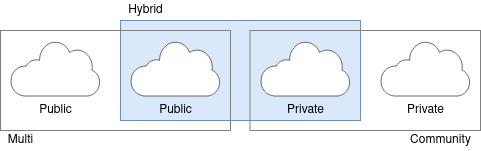
\includegraphics[width=.8\linewidth]{img/def_cloud_models_v2.png}
        \captionsetup{justification=centering}
        \caption{
             \Gls{hybrid_cloud}  combines public and \glspl{private_cloud} (middle box), whereas using multiple \glspl{public_cloud} is referred to as \gls{multi_cloud} (left box).
            Sharing \glspl{private_cloud} is known as \gls{community_cloud} (right box).
        }
        \label{fig:cloud-models}
    \end{figure}

     \Gls{hybrid_cloud}  models tend to be heterogeneous in nature, due to the fact that two different, usually unrelated companies are handling operations.
    However, this model offers a good mix of control and scalability, profiting from high elasticity of \gls{public_cloud} providers and high flexibility of \gls{private_cloud} installations.
    Many concepts that work for \gls{hybrid_cloud} can also be applied to \glsdisp{multi_cloud}{multi} or \gls{community_cloud} models, however, those models will not be further elaborated in this thesis.

    \Gls{cloud} models and patterns are currently an active area of research.
     \Gls{hybrid_cloud}  was suggested to give the best economic value\cite{policy_hc_deploy} and enterprise adoption is driven by the expectation to achieve cost savings\cite{hc_patterns}.
    For businesses with restrictions on where data is stored it is a good choice to be in control of the data location but still profit from the elasticity of the \gls{public_cloud} for services that are less location-critical\cite{policy_hc_deploy}.

    A \gls{hybrid_cloud} setup comes with new possibilities and challenges, for which architectural patterns have emerged\cite{hc_patterns}:
    \begin{itemize}
        \setlength\itemsep{0em}
        \item \textbf{Static placement}, where workloads are strongly bound to one \gls{cloud} and might not be able to run on the other
        \item \textbf{Assisted replication}, where workloads are replicated from one \gls{cloud} to the other
        \item \textbf{Automigration}, where workloads are moved from one \gls{cloud} to the other by a tool or through human intervention
        \item \textbf{Dynamic migration}, where workloads are moved between \glspl{cloud} dynamically, which may include scaling workloads across \glspl{cloud}
    \end{itemize}

     Many studies have been conducted in this ongoing field of research on deployments based on data location\cite{policy_hc_deploy}, \gls{cloud} interoperability\cite{policy_driven_hc_mw} and workload orchestration for high availability\cite{orchestrating_ha_deployment} or in the presence of failures\cite{rc_prov_policy_failures,failure_aware_placement}.
    Also, on the migration of workloads based on virtual machines\cite{policy_mc_migr} or container orchestration platforms\cite{rw_migr_cloud_apps}.
    Still, challenges remain around deploying and migrating effectively.

    With any combination of \glspl{cloud}, the need arises for management solutions and abstractions to handle governance, billing and resource management, including development, deployment, testing and monitoring but also optimizations for usage and pricing.\cite{rw_comparison_mcmp}

    \subsubsection{Cloud service models}
    \label{subsubsec:defs-cloud-service-model}

    The main services that \glspl{cloud} offer are \acrfull{iaas}, \acrfull{paas}, \acrfull{faas} and \acrfull{saas}\@.
    They are defined as\cite{cloud_def_nist,cloud_def_nist_eval,faas_status}:
    \begin{itemize}
        \setlength\itemsep{0em}
        \item \textbf{\acrshort{iaas}} is the capability of provisioning infrastructure including computing, storage and network
        \item \textbf{\acrshort{paas}} is the capability of deploying applications using various languages, libraries and services provided without having to manage the underlying infrastructure
        \item \textbf{\acrshort{faas}} is the capability of running code functions without having to manage the application runtime, which is also referred to as serverless computing
        \item \textbf{\acrshort{saas}} is the capability of using and configuring software without having to manage the applications or infrastructure used to provision it
    \end{itemize}

    \acrshort{paas}-level \glspl{cloud} are coming with a lot of support to ease development and deployment of applications and promote \gls{devops} tools and practices.
    The benefits of simple deployments and dynamic scalability usually comes with reduced flexibility and portability to allow vendors to manage capacity and availability of services.\cite{cd_cloud_computing}

    Many commercial and non-commercial \acrshort{paas} platforms are available today, some of which run on top of existing \acrshort{paas} and \acrshort{iaas}\cite{paas_players}.
    Work has been conducted to build federated \acrshort{paas} systems\cite{federated_paas} or further abstract \gls{java}-based \acrshort{paas} platforms\cite{policy_driven_hc_mw} to improve portability.

    The current lack of standardization and problems of reduced control and portability of \acrshort{paas} platforms are often causing a vendor lock-in.
    Although \acrshort{paas} will be a key deployment model going forward, this remains a risk for enterprises adopting platform services.\cite{gartner_paas_trends}

    \subsubsection{Cloud-native applications}
    \label{subsubsec:cloud-native}

    \Gls{cloud_native} is a design principle.
    \Gls{cloud_native} applications are built with failure tolerance in mind.
    They are redundant, adaptive, and can cope with changes in the underlying infrastructure.
    In addition, they are dynamically scalable if the load from incoming requests changes.
    Often, they are highly distributed and following a modular, microservice architecture.
    A good analogy is that \gls{cloud_native} applications have to be more stable than the infrastructure they are running on.\cite{cna_patterns,cn_devops_with_k8s_c1}

    In contrast, non-\gls{cloud_native}, legacy applications have certain attributes that make it undesirable or even impossible to containerize and run as ephemeral units.
    If a monolithic application with a long startup time does not scale and is mission critical, the underlying hardware has to be very stable and rescheduling is not feasible unless absolutely necessary.
    Additional restrictions apply for certain communication models, such as multicast, which is not always supported by the underlying network in \gls{cloud} environments.
    There are tools available that enable multicast by emulating a layer 2 network.
    However, this might not always be desirable as it creates another layer of complexity and adds a dependency on third-party software.\cite{cna_patterns,cloud_multicast}

    \subsection{DevOps}
    \label{subsec:devops}

    \gls{devops} has gained a lot of momentum recently.
    The main aim of \gls{devops} is to bring development and operations closer together.
    Looking at it from that perspective, it is strongly driven by communication.
    In practice, \gls{devops} is a set of tools and practices that enables companies to promote the right culture and increase the efficiency of their \acrlong{sdlc}.\cite{cn_devops_with_k8s_c1,devops_surveys}

    \gls{devops} has a rich research literature and State of \gls{devops} Reports are published annually with survey data from many organisations in the industry.
    The two pillars of \gls{devops} have been defined as collaborative culture and automation\cite{devops_real_world,devops_surveys} and the three main principles as flow, feedback and continuous learning and experimentation\cite{devops_handbook_1}.

    Deploying and assessing quality of \gls{devops} practices in organisations, qualification of engineers and redesigning system for continuous delivery remain the biggest challenges\cite{devops_surveys}.
    It means acquiring new skills for both software developers and system administrators, convincing senior managers and fully automating the deployment process in complex environments, while coping with existing legacy technology\cite{devops_multicase}.
    Other pitfalls are manual steps throughout the process, capacity bottlenecks and not having environment parity\cite{devops_pitfalls}.

    There is no single, correct instruction for adoption but rather a set of topologies and best practices that can be worked with.
    Companies would often have to change their communication structure to successfully operate \gls{devops}.
    As a result, many anti-types are forming as per Conway's law, which says that systems within an organisation mirror their communication structure.\cite{devops_topologies}

    \subsubsection{DevOps interpretations}
    \label{subsubsec:defs-devops}

    The term \gls{devops} is a combination of development (Dev) and operations (Ops).
    This includes the field of quality assurance (Fig.~\ref{fig:devops_venn}).
    It has a lot in common with \acrlong{sre} at Google, which predates \gls{devops} but could be seen as an implementation of it\cite{sre_google}.

    \begin{figure}[h]
        \centering
        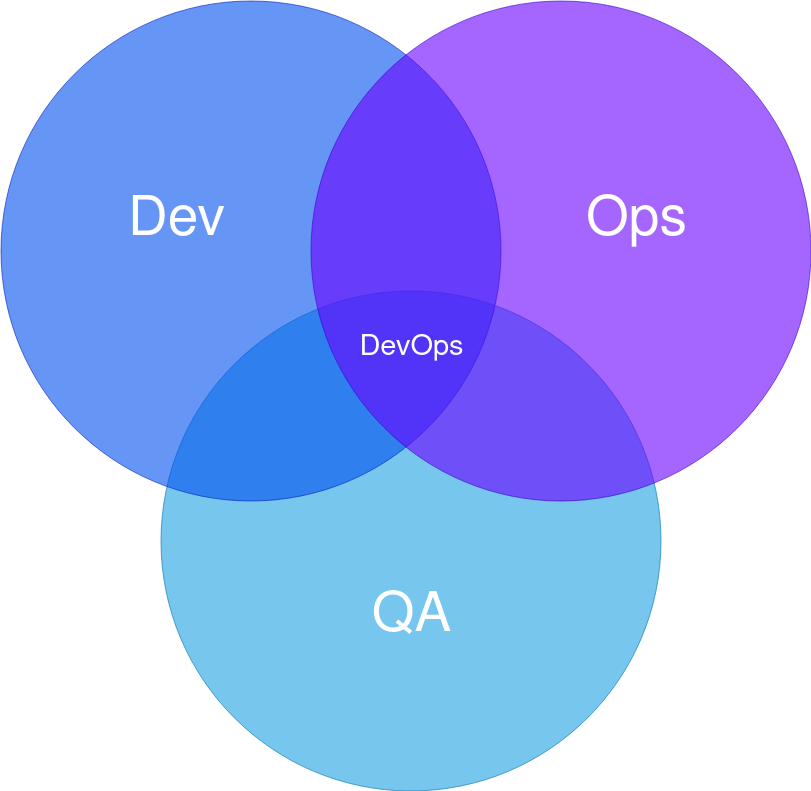
\includegraphics[width=.6\linewidth]{img/def_devops_venn_v3.png}
        \captionsetup{justification=centering}
        \caption{
        Development (Dev), operations (Ops) and quality assurance (QA) forming \gls{devops}.
        }
        \label{fig:devops_venn}
    \end{figure}

    Over time, different interpretations have formed many variants.
    Starting from \gls{devops}, all variants can be grouped by specification and automation (Fig.~\ref{fig:devops_spec}).
    \gls{devsecops} is a more recent evolvement that aims to explicitly capture security in the model.
    \gls{bizdevops} tries to bring \acrshort{it} and business closer together.
    \gls{archops} sets additional emphasis on analysis and design on an architectural level with feedback from automated monitoring.
    \gls{winops} is built around the world of Microsoft Windows.
    \gls{testops} is an attempt to port \gls{devops} principles onto hardware manufacturing and electronic design automation.
    In the field of data science, \gls{dataops} is used for data engineering, management and business intelligence.
    Further, \gls{aiops} is meant to help with operations processes by evaluating and learning based on the available data from monitoring.
    With \gls{noops}, classical operations is completely factored out.
    It could be argued if this is in line with \gls{devops} principles but it is something that can be achieved with \acrshort{paas}-level \glspl{cloud}.\cite{winops,testops,devsecops,archops,dataops,aiops,noops,bizdevops}

%    make it look like the gartner quadrants

    \begin{figure}[h]
        \centering
        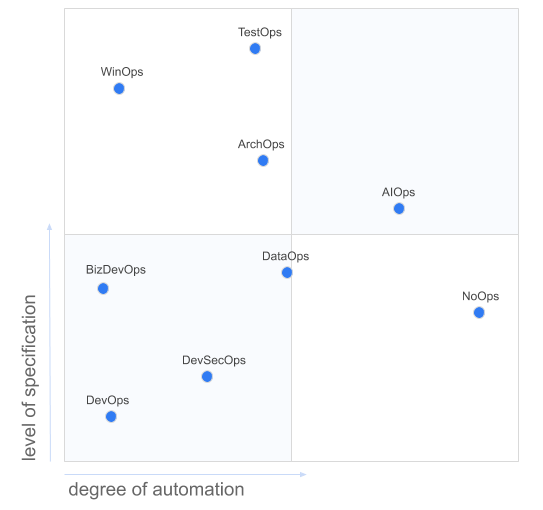
\includegraphics[width=.9\linewidth]{img/def_devops_quadrant_v3.png}
        \captionsetup{justification=centering}
        \caption{
        Quadrant of \gls{devops} interpretations classifying \gls{devops} variants by specification and automation, based on an estimation by the author.
        The variants are \gls{devops}, \gls{devsecops}, \gls{bizdevops}, \gls{dataops}, \gls{archops}, \gls{winops}, \gls{testops}, \gls{aiops} and \gls{noops}.
        }
        \label{fig:devops_spec}
    \end{figure}

    \subsubsection{Stages of DevOps}
    \label{subsubsec:defs-toolchain}

    While \gls{devops} is a set of principles, it is usually referred to as a set of stages, forming the \gls{devops} toolchain.
    A common way of visualising the \gls{devops} toolchain is the \gls{devops} loop (Fig.~\ref{fig:devops_loop}).

    \begin{figure}[h]
        \centering
        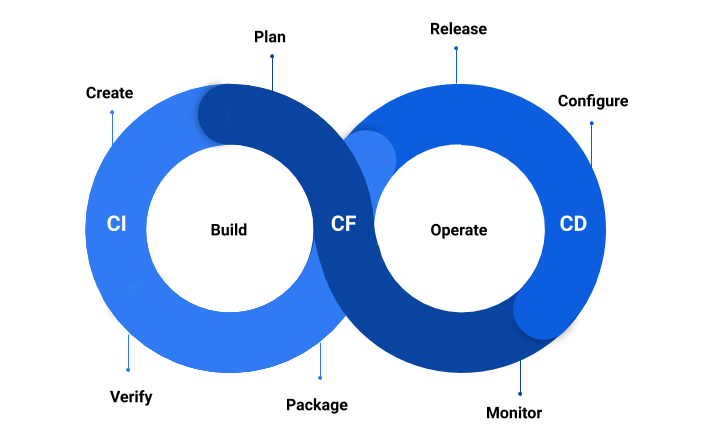
\includegraphics[width=.99\linewidth]{img/def_devops_loop_v3.png}
        \captionsetup{justification=centering}
        \caption{
            \gls{devops} toolchain with the stages plan, create, verify, package, release, configure and monitor to achieve \acrfull{ci}, \acrfull{cd} and \gls{cont_feed} (CF).
        }
        \label{fig:devops_loop}
    \end{figure}

    Although it comes down to the same practices, the \gls{devops} stages are not defined consistently.
    It appears that companies that are more involved with \gls{cloud} consultancy tend to favour terms that are more readily understood due to its widespread use in technology reports and books.

    Atlassian defines the stages as plan, build, continuous integration, continuous deployment, monitor, operate and continuous feedback.
    Microsoft replaces continuous deployment and monitor with a single stage, deploy.
    In contrast, Amazon, Splunk and GitLab prefer to use a finer-grained specification of plan, create, verify, package, release, configure and monitor.
    Each definition has collaboration and communication at its core and version control as a common denominator for all stages.
    A definition for the stages is derived as\cite{what_is_devops_atlassian,what_is_devops_microsoft,what_is_devops_aws,what_is_devops_splunk,what_is_devops_gitlab}:

    \begin{itemize}
        \setlength\itemsep{0em}
        \item \textbf{Plan} and document the requirements, draw conclusions and learn from previous cycles
        \item \textbf{Create}, design, implement and improve the software product
        \item \textbf{Verify} the change with acceptance tests, scan for quality issues and security vulnerabilities
        \item \textbf{Package} into shippable, traceable units, control versions and dependencies
        \item \textbf{Release} to production systems, following the sign-off processes
        \item \textbf{Configure} external dependencies and establish the required links among services
        \item \textbf{Monitor} the environment, gather metrics and insights and alert on misbehaviour
    \end{itemize}

    In other words, the goal is to build and operate software which is best achieved through \acrfull{ci}, \acrfull{cd} and \gls{cont_feed}, all of which play their part in \gls{cont_del} and are key to \gls{devops}.

    This thesis is primarily concerned with concepts around package and release to enable \acrlong{cd} into \gls{hybrid_cloud} environments.

\end{document}

